%!TEX root = main.tex
% we developed features that addresses the challenges they pose on VQSs, described first in this section. From these experiences, we develop a taxonomy for summarizing key functionalities in VQSs.
% From participatory design,
\begin{figure*}[ht!]
  \centering
  \vspace{-5pt}
  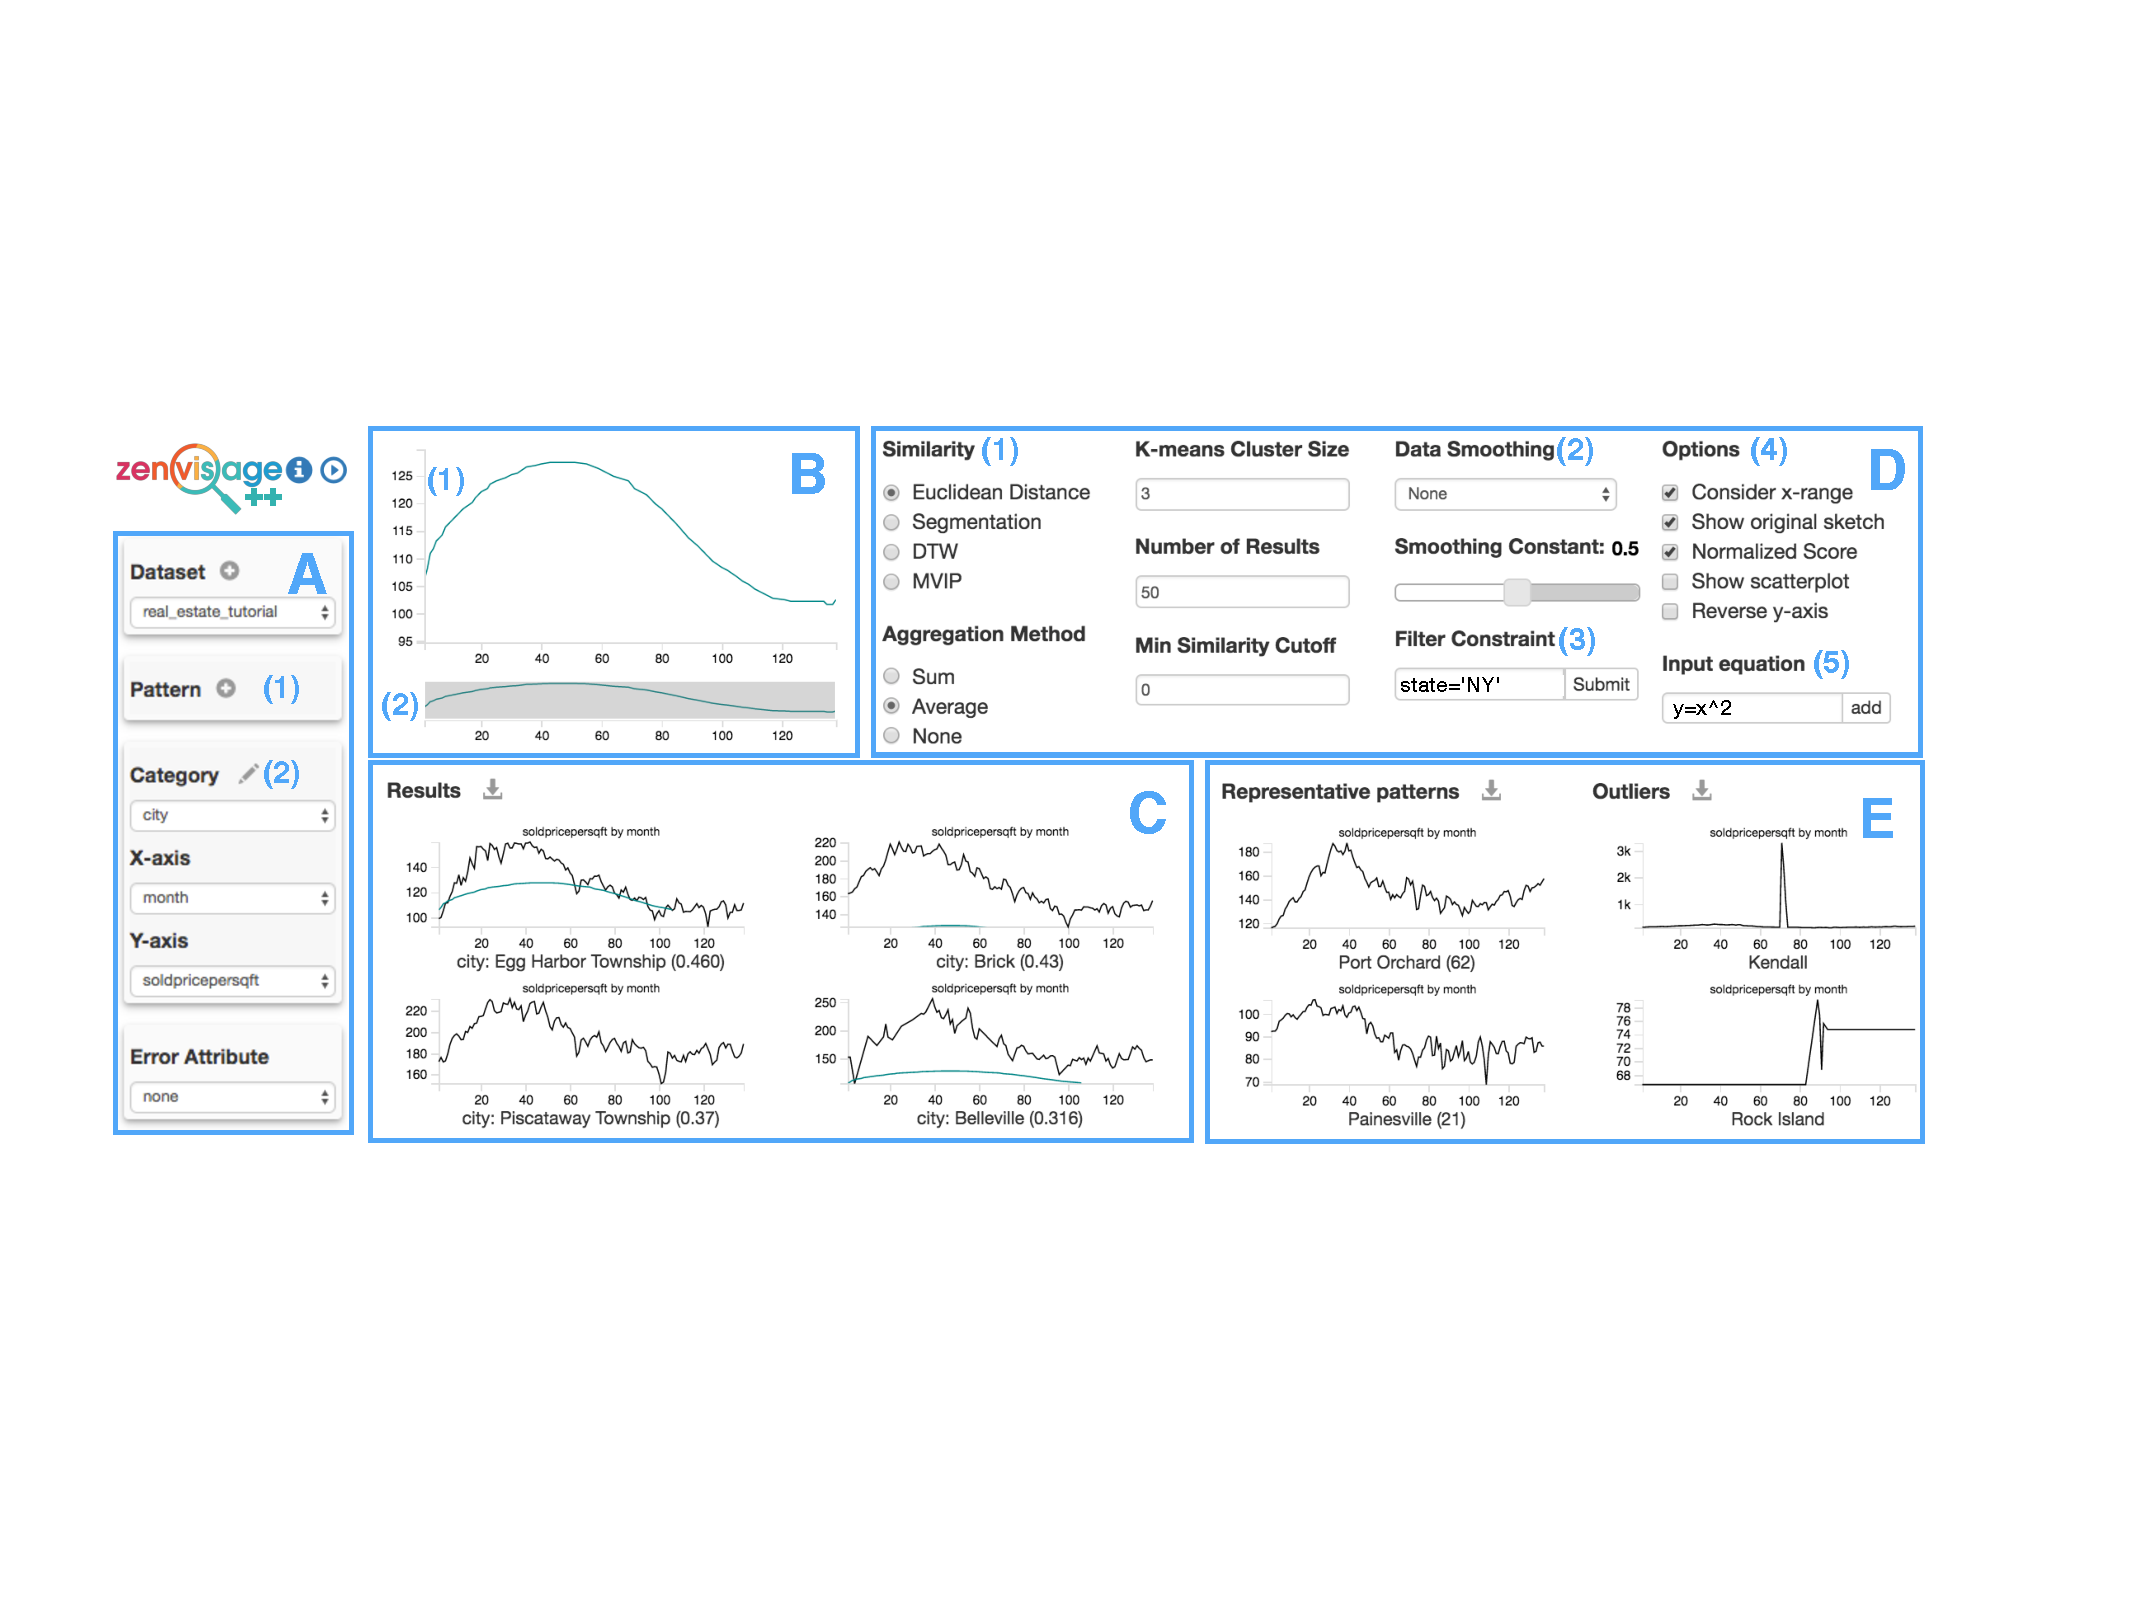
\includegraphics[width=0.95\linewidth]{figures/zvpp_system.pdf} %5.5
  \vspace{-5pt}\caption{\change{The \zvpp system consist of : (A) data selection panel (where users can select visualized dataset and attributes), (B) query canvas (where the queried data pattern is submitted and displayed), (C) results panel (where the visualizations most similar to the queried pattern is displayed as a ranked list), (D) control panel (where users can adjust various system-level settings), and (E) recommendation (where the typical and outlying trends in the dataset is displayed).}} %Prior to the participatory design, \zv only included a single sketch input with no additional options.}
  %the ability to query via (a) a sketch,(b) input equations, (i) uploaded patterns, or (j) drag and drop; (c) data smoothing; query specification mechanisms including (d) x-range selection and filtering, (e) x-range invariance, (f) similarity metric selection, (g) filtering, and (h) dynamic class creation; recommendation of (k) representative and (l) outlier trends.
  \label{zvOverview}
  \vspace{-5pt}
\end{figure*}
\section{Participatory Design Findings\label{sec:pd_findings}}
All of the three domains described in the previous section recognized the need for a VQS. As discussed in Section~\ref{sec:methods}, we worked closely with participants to develop features to address their problems and challenges. \change{In this section, we first provide a high-level system overview of \zvpp. Through our participatory design findings,} we develop a taxonomy for organizing these functionalities into three sensemaking processes, as shown in Figure~\ref{fig:taxonomy}. %We first describe features that we incorporated into our enhanced VQS, \zvpp, thematically organized by components (grouping features in the bottom-most level to components in the second level of Figure~\ref{fig:taxonomy}).
\change{Starting from the bottom level of the taxonomy, we first describe what each component in our taxonomy encompasses, then we proceed onto the upper level of the taxonomy, describing the space of problems addressable by each sensemaking process and their design objectives.}%collaboratively-designed
%Next, we describe features that we incorporated into our enhanced VQS, \zvpp, thematically organized by component. Then, we introduce a taxonomy for organizing these components into three sensemaking processes, spanning different problem areas that VQSs are aimed to solve.
%\change{In this section, we will first introduce a taxonomy for organizing these components into}
%Based on feature requests and discussion with our participants, we incorporated key features missing in our original VQS.
%From these discussion and analysis of past VQSs, we identify nine components of VQSs, described below. T
% Along with analysis of past literature, we develop a taxonomy of key functionalities in VQSs.
% novel contribution on  ---
% contribute to holistic understanding on how sensemaking --- in VQS.
% study on how users
% Implication ---
% •	What types of questions/ dataset/ problem challenges are asked to VQS or can be addressed by VQS? (S3)
% •	What kind of features needs to be designed to address these challenges (S4 PD)
%We employed participatory design with our scientists to incorporate key features missing in our original VQS, and unaddressed in their existing workflows. From these discussion and analysis of past VQSs, we identify nine components of VQSs, described below.
\begin{figure*}[ht!]
  \centering
  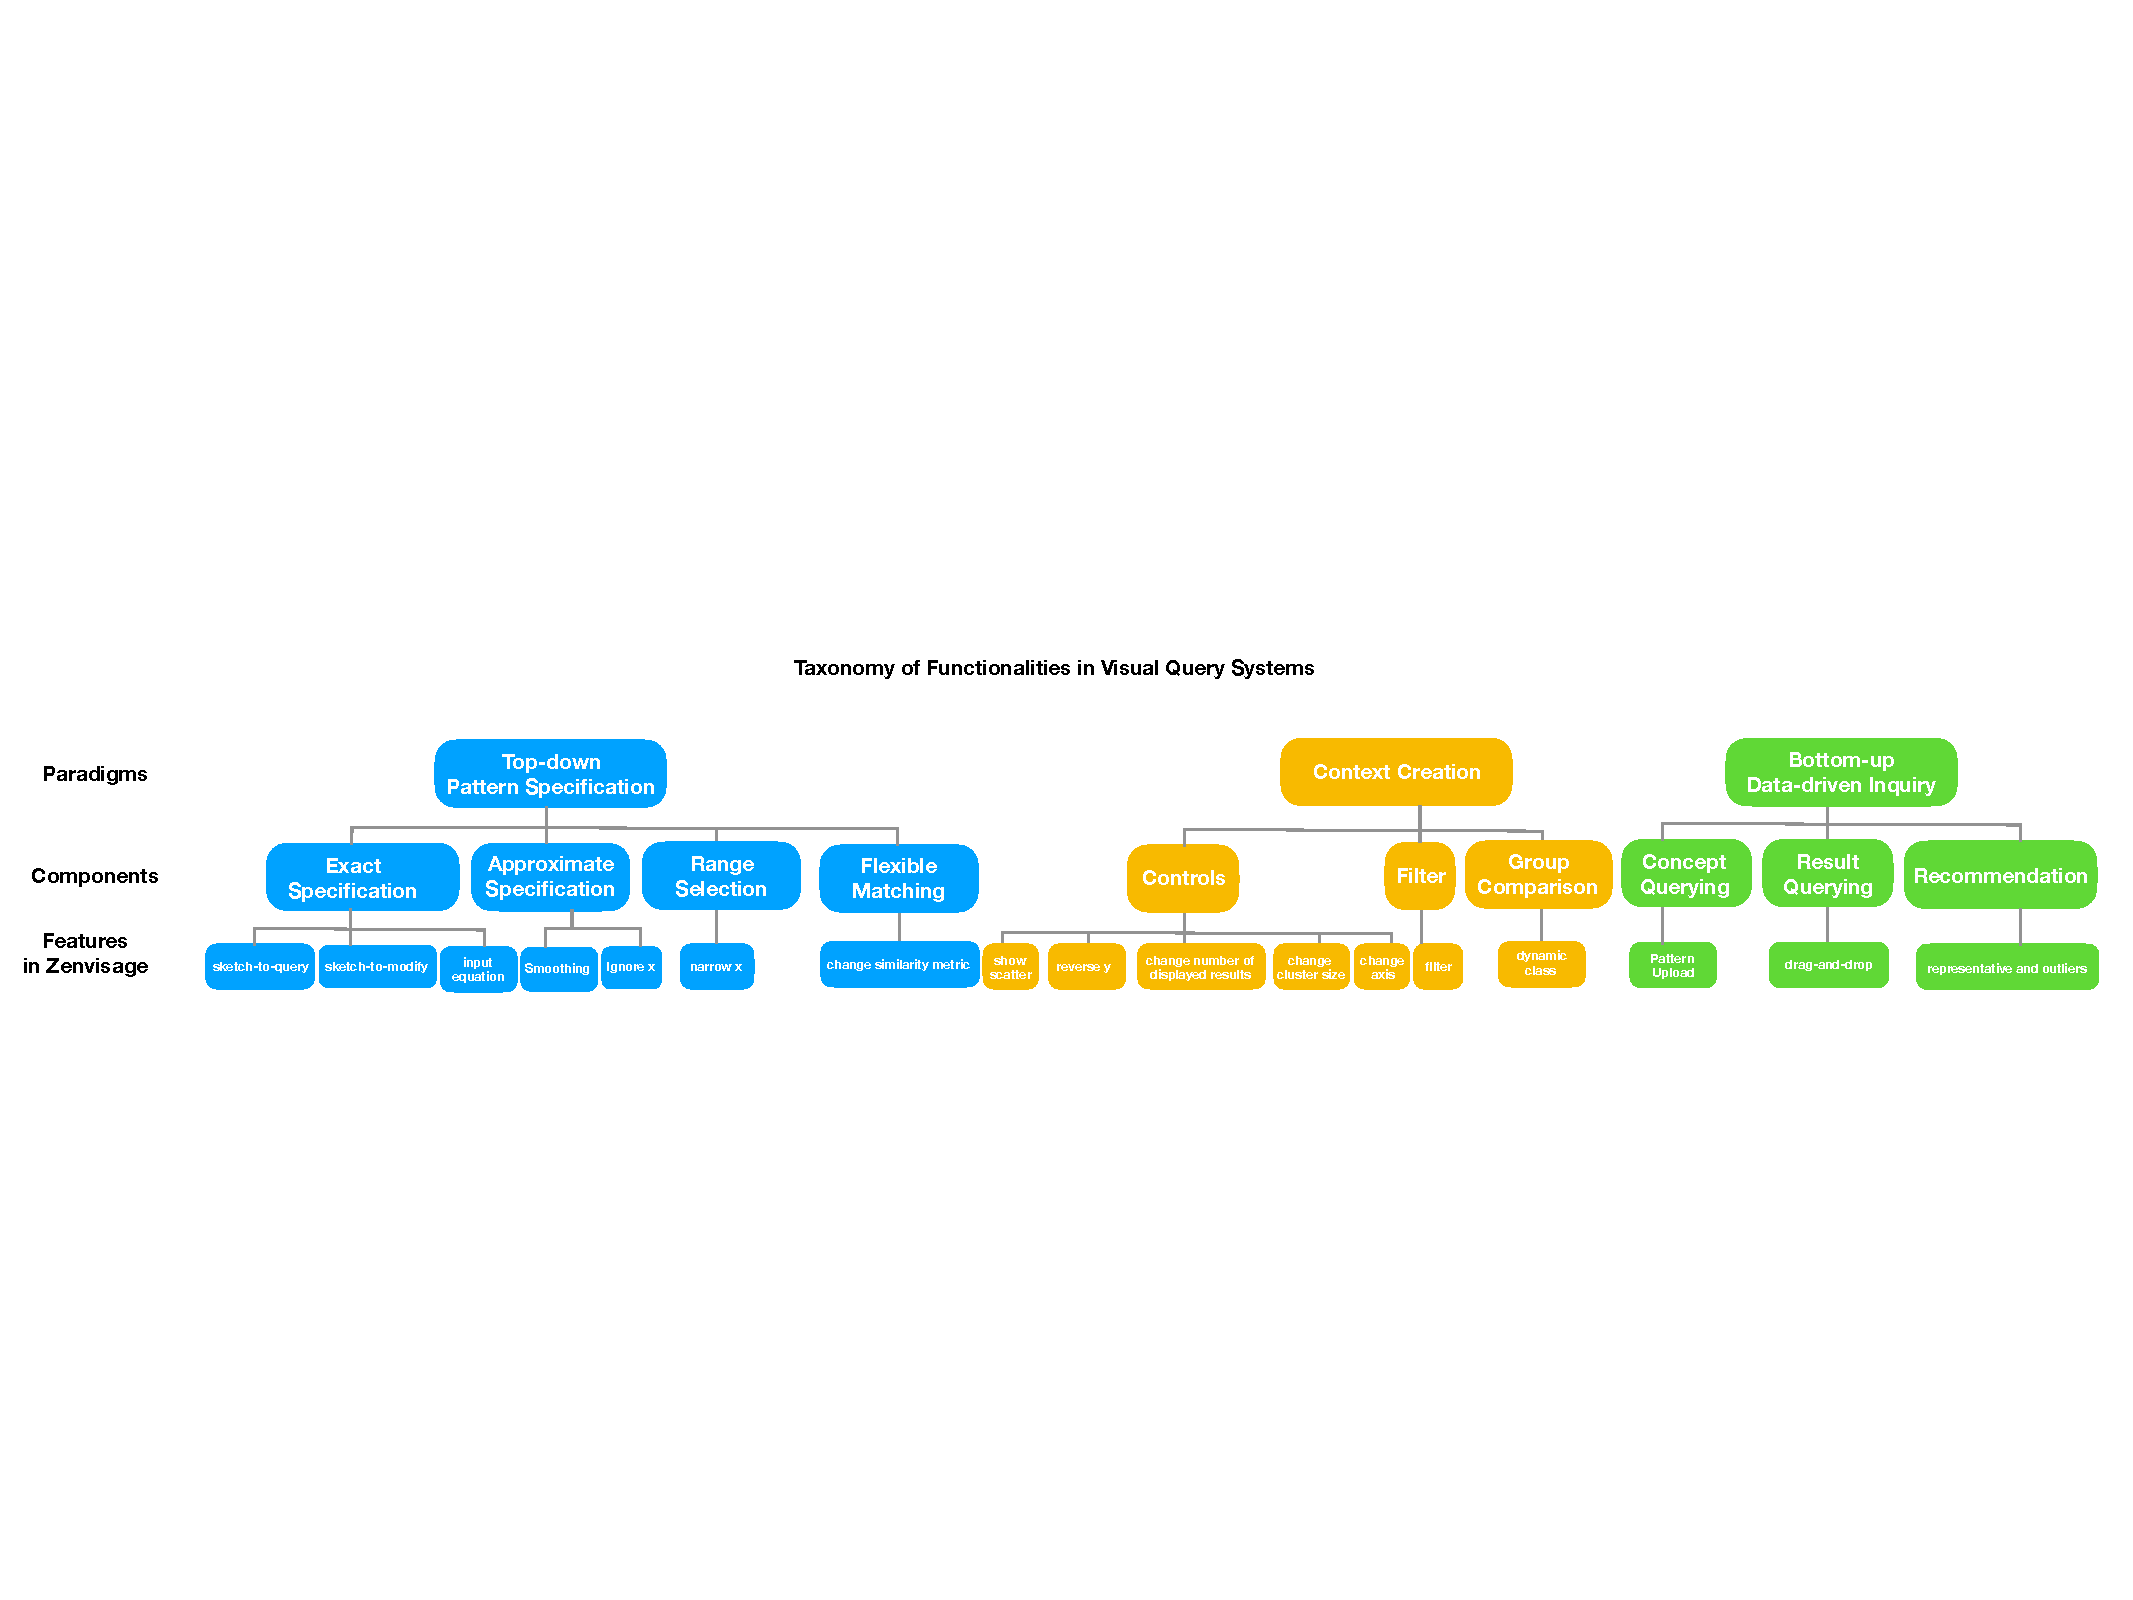
\includegraphics[width=0.9\linewidth]{figures/taxonomy.pdf}
  \caption{Taxonomy of functionalities in VQSs. Each of the three sensemaking process is broken down into key functional components in VQSs. \change{We list the types of questions addressed by each component from a system's perspective.}} %, which is instantiated as features in \zvpp.}% The bottom-most layer connects the use cases features that have practical or envisioned usage based on the evaluation study.}
  \label{fig:taxonomy}
\end{figure*}
\change{
  \subsection{System\label{sec:system}}
  The \zvpp interface is organized into 5 major regions that dynamically updates upon user interactions. Typically, analysts begin their analysis by selecting the dataset and attribute to visualize in the \emph{data selection panel} (Figure~\ref{zvOverview}A). Then, they can specify a pattern query of interest, through either sketching, inputting an equation, uploading a data pattern, or dragging and dropping an existing visualization, displayed on the \emph{query canvas} (Figure~\ref{zvOverview}B). \zvpp performs shape-matching between the queried pattern and other possible visualizations and returns a ranked list of visualizations that are most similar to the queried pattern, displayed in the \emph{results panel} (Figure~\ref{zvOverview}C). At any point during the analysis, analysts can adjust various system-level settings through the \emph{control panel} (Figure~\ref{zvOverview}D) or browse through the list of \emph{recommendations} provided by \zvpp (Figure~\ref{zvOverview}E). Our \zvpp system is open source and available at: \url{github.com/[Annonymized for Submission]}.
}
\subsection{\change{Components} Emerging from Participatory Design\label{sec:pd_findings}}
\change{
  Here, we discuss the purpose of the components in the lower-level of our Figure~\ref{fig:taxonomy} taxonomy, motivating use cases collected over the course of participatory design, and how these themes instantiate into corresponding features in \zvpp and other existing VQSs. Each of the features described (labelled F*) correspond directly to a use case challenge (labelled C*) highlighted in the list above it.
}
\subsection{Reflection on Meta-Design Process}
